\newpage
\section{Forze}
La legge oraria $\vec{F}(t)$ di un punto materiale di massa m è determinata salla soluzione di una equzione
del moto detta \textbf{seconda legge di newton}
$$m\ddot{\vec{r}} = \vec{F}_1 + \vec{F}_2 + \dots$$
$\vec{F}_1$ sono le \textbf{forze} $[kg \cdot m/s^2 \equiv N]$ (N è l'unità di misura, Newton) agenti sul punto meteriale: sono determinate empiricamente.
L'equazione differenziale è del \textbf{secondo ordine} (derivata seconda) quindi servono due \textbf{condizioni al bordo} (si chiamano così perché indicano le 
condizioni ai bordi del dominio), ad esempio $\vec{r}(t_0) = \vec{r}_0$ e $\dot{\vec{r}}(t_0) = \vec{v}_0$ (con questa cosa stiamo dicendo che per decsrivere un moto di un sistema
dobbiamo sapere in un tempo dove il sistema si trova e la sua velocità).\\
Questa è un equazione che va a descrivere fenomeni da dimensioni incredibilmente piccole a incredibilmente grandi.\\\\
Se la somma (detta \textbf{risultate} delle forze)
$$\vec{F}_1 + \vec{F}_2 + \cdots = 0 \hspace{10pt}\text{allora}\hspace{10pt} m\ddot{\vec{r}}(t) = 0 \Rightarrow \dot{\vec{v}}(t) \equiv \vec{v}_0$$
cioè il moto ha velocità costante (\textbf{rettilineo uniforme}). Questo è in particolare vero se tutte $\vec{F}_i = 0$ 
(\textbf{prima legge di Newton} o "principio di inserzia di Galileo"). Se un corpo non è soggetto a forze esterne mantiene il suo modo rettilineo uniforme.
Questa cosa collega la proprierà di simmetria degli oggetti alla traslazione dello spazio.

\subsection{Forza costante $\vec{F} = F_0\hat{x}$}
$$\vec{r}(t) = x(t)\hat{x} + y(t)\hat{y} + z(t)\hat{z} \hspace{15pt}\ddot{\vec{r}}(t) = \ddot{x}(t)\hat{x} + \ddot{y}(t)\hat{y} + \ddot{z}(t)\hat{z}$$
$$m\ddot{\vec{r}}(t) = F_0 \hat{x} \Rightarrow 
\begin{cases}
    m\ddot{x}(t) = F_0\\
    m\ddot{y}(t) = 0\\
    m\ddot{y}(t) = 0 
\end{cases}
$$
Proietto su una base per ottenere 3 equazioni scalari. Mi servono $2 \times 3 = 6$ \textbf{condizioni al bordo} per risolvere.
Ad esempio condizioni iniziali:
$$\vec{r}(0) = \vec{r_0} = (x_0, y_0, z_0) \hspace{15pt} \dot{\vec{r}}(0) = \vec{v}_0 = (v_{0x}, v_{0y}, v_{0z})$$
$$\Rightarrow 
\begin{cases}
    x(t) = x_0 + v_{0x}t + \frac{1}{2}\frac{F_0}{m}t^2\\
    y(t) = y_0 + v_{0y}t \\
    z(t) = z_0 + v_{0z}t
\end{cases}
\Rightarrow \:\:\text{caso generale}\:\:
r(t) = r_0 + v_0t + \frac{1}{2}\frac{F_0}{m}t^2
$$
Con $t$ che rappresenta il \textbf{moto uniformamente accelerato}

\subsection{Forza peso $\vec{F} = -mg\hat{z}$}
Usata per esempio in prossimità della superficie terreste. Con $m$ massa del punto materiale dell'oggetto in cui si applica, mentre $\hat{z}$ ortogonale alla superficie. 
$g \equiv 9,8 m/s^2$, dipende da $M_T$, variazioni locali.
\begin{example}
    Grave che cade da altezza $h$.
    $$m\ddot{\vec{r}}(r) = -mg\hat{z} \hspace{15pt} \text{con}\hspace{15pt} \vec{r}(t_0) = h \cdot \hat{z}, \dot{\vec{r}}(t_0) = 0 \text{(oggetto parte da fermo)}$$
    Proietto $m\ddot{z}(t)= -mg$ \hspace{10pt} $\dot{z}(t) = -g(t - t_0)$ \hspace{10pt} $z(t) = h - \frac{1}{2}g(t - t_0)^2$\\
    Si sostituisce le costanti della soluzione per verificare che siano verificate le condizioni ai bordi.
\end{example}

\begin{example}
    Problema del proiettile.
    $$m\ddot{\vec{r}}(t) = -mg\hat{z} \:\:\text{(equazione del moto)}\:\:\: \text{con} \:\:\vec{r}(t_0) = 0$$
    $$\text{e}\:\: \dot{\vec{r}}(t_0) = v_0 \cdot \cos\Theta\hat{x} + v_0 \cdot \sin\Theta\hat{z} \hspace{10pt}\text{ovver}\hspace{10pt}\vec{v}_0 = v_0(\cos\Theta, \sin\Theta) \:\: ||\vec{v}_0|| = v_0$$
    Qui andiamo a considerare quindi una certa velocità $v_0$ con un angolo $\Theta$, e andiamo a definire la vecolità $\vec{v}_0$.
    Proiezione lungo $\hat{y}$ banale: $\ddot{y}(t) \equiv 0, y(t) \equiv 0$
    $$
    \begin{cases}
        \ddot{x}(t) = 0& \hspace{20pt} \dot{x}(t) = v_0 \cos\Theta \\
        \dot{x}(t_0) = v_0 \cos\Theta & \hspace{20pt} x(t) = v_0\cos\Theta (t-t_0)\\
    \end{cases}
    $$
    $$
    \begin{cases}
        \ddot{z}(t) = -g & \hspace{20pt} \dot{z} = v_0 \sin\Theta - g(t - t_0)\\
        \dot{z}(t_0) = v_0 \sin\Theta & \hspace{20pt} z(t) = v_0\sin\Theta(t - t_0) - \frac{1}{2}g (t - t_0)^2
    \end{cases}
    $$
    Dalla legge oraria alla traiettoria
    $$
    \begin{cases}
        x(t) = v_0 \cos\Theta(t - t_0)\\
        z(t) = v_0\sin\Theta(t - t_0) - \frac{1}{2}g(t - t_0)^2
    \end{cases}
    $$
    $$t - t_0 = x(t) \: / \: (v_0\cos\Theta) \hspace{10pt} z = v_0\sin\Theta x\: / \: (v_0 \cos\Theta) - \frac{1}{2}g x^2 \: / \: (v_0\cos\Theta)^2 \hspace{10pt} z=v_0 tg\Theta - x^2 \frac{g}{2v_0^2}\frac{1}{\cos^2\Theta}$$
    \begin{observation}
        $\frac{1}{\cos^2\Theta} = \frac{\sin^2\Theta + \cos^2\Theta}{\cos^2\Theta} = 1 + tg^2\Theta \hspace{15pt} z = x tg\Theta - x^2 \frac{g}{v_0^2}(1 + tg^2 \Theta)$ (Parabola)
    \end{observation}
    \hspace{-15pt}Punto di atterraggio: sistema con $z = 0$, $x = 0$ (banale) \hspace{10pt} $x = \frac{2v^2_0}{g}tg\Theta / (1 + tg^2 \Theta)$
\end{example}
\begin{figure}[h!]
    \centering
    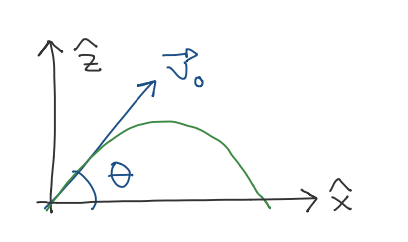
\includegraphics[width=0.3\textwidth]{images/esempio-proiettile.png}
    \caption*{Esempio proiettile}
\end{figure}

\subsection{Forza elastica $\vec{F} = -k (||\vec{r} - \vec{r}_v|| - l_0)\frac{\vec{r}-\vec{r}_v}{||\vec{r}-\vec{r}_v||}$}
\begin{wrapfigure}[7]{r}{4cm}
    \vspace{-15pt}
    \centering
    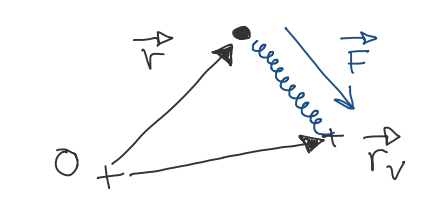
\includegraphics[width=5cm]{images/forza-elastica.png}
\end{wrapfigure}
Chiamata anche \textbf{legge di hooke}. $k$ è la costante elastica espressa in $[N/m]$ del materiale. $l_0 [m]$ lunghezza a riposo della "molla", 
dipende dal vettore posizione $\vec{r}$ ("posizionale").\\\\
$-\frac{\vec{r}-\vec{r}_v}{||\vec{r}-\vec{r}_v||}$ è il versone parallelo alla molla, cioò la distanza fra il punto di destinazione ed il vincolo, si usa perché c consente
di calcolare la forza elstica $F$ nella direzione esatta della deformazione, anziché utilizzare solo la magnitudo della deformazione ($(||\vec{r} - \vec{r}_v|| - l_0)$).
\\\\La forza elastica è tanto piu intensa quanto è estesa la molla, e questa relazione fondamentale è lineare. Una versione
più classica della legge di hooke è:
$$\vec{F} = kx$$
\begin{example}
    Oscillatore unidimensionale $\vec{r}_v = 0$.
    $$\vec{r}(t) = x(t)\vec{x}, \:\:\:x(t)\geq 0$$
    $$\vec{F}= -k(|x-0| - l_0)\frac{x - 0}{|x - 0|}\hat{x} \hspace{10pt} = \hspace{10pt} -k(|x| - l_0)\frac{x}{|x|}\hat{x} \Rightarrow F_x = -k(x-l_0)$$
    $$m\ddot{x}(t) = -k[x(t) - l_0]$$
    Soluzione generale (verifico per sostituzione)
    $$x(t) = l_0 + A \cdot \cos(\Omega t) + B \cdot \sin(\Omega t) \hspace{15pt} \Omega \equiv \sqrt{k/m}$$
    $$\dot{x}(t) = -\Omega A \sin(\Omega t) + B \Omega \cos(\Omega t)$$
    $$\Omega[rad/s] \text{la \textbf{frequenza angolare}} \hspace{10pt} \Omega/2\pi [\frac{1}{s} = Hz] \text{è la \textbf{frequenza}} \hspace{10pt} T = 2\pi/\Omega [s] \text{è il \textbf{periodo}, infatti } \Omega \cdot T = 2\pi$$ 
    Trovo $A$ e $B$ imponendo che la soluzione rispetti le condizoni al bordo, es: $x(0) = x_0, \dot{x}(0) = 0$. 
    Dalla soluzione generale ho 
    \begin{align*}
        & \dot{x}(t) = -\Omega A \sin(\Omega t) + B \Omega \cos(\Omega t) \:\: \xrightarrow{b.} \:\: 0 = -\Omega A \sin(\Omega \cdot 0) + B \Omega \cos(\Omega \cdot 0) \:\:\rightarrow\:\: 0 = 0 + B\Omega \Rightarrow B = 0\\
        & x(t) = l_0 + A \cdot \cos(\Omega t) \:\:\xrightarrow{a.}\:\: x_0 = l_0 + A \cdot \cos(\Omega \cdot 0) \:\:\rightarrow\:\: x_0 = l_0 + A
    \end{align*}
    La soluzione completa è quindi
    $$x(t) = l_0 + (x_0 - l_0) \cos(\Omega t)$$
\end{example}

\subsection{Forza di attrito viscoso $\vec{F} = -\gamma\dot{\vec{r}}(t)$}
Modello approssimato per le basse velocità. Abbiamo che $-\gamma [N/(m/s)]$ è la costante del materiale viscoso. Il meno è dato perché è una forza
che si oppone linearmente ad una velocità.
\begin{example}
    Proiettile in gel balistico.
    $$m\ddot{x}(t) = \gamma t \dot{x}(t) \:\: con \:\: \dot{x}(0) = v_0$$
    Pongo poi $u(t) \equiv \dot{x}(t) \Rightarrow \dot{u} t = -\frac{1}{\tau}u(t)$ con $u(0) = v_0$ e $\frac{1}{\tau} = \frac{\gamma}{m}[\frac{1}{s}]$\\
    Soluzione generale $u(t) = A e^{-t/\tau} \Rightarrow v_0 = A \cdot e^0 \Rightarrow v_0 = A$.\\
    Quindi la soluzione completa è
    $$u(t) = v_0 e^{-t/\tau} \:\:\: \text{ovver} \:\:\: \dot{x}(t) = v_0 e^{-t/\tau}$$
    rallentamento esponenziale.
\end{example}
\begin{figure}[h!]
    \centering
    \begin{subfigure}[b]{0.3\textwidth}
        \centering
        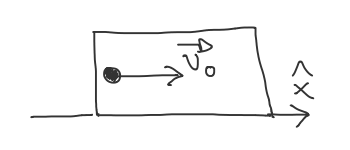
\includegraphics[width=\textwidth]{images/proiettile-gel-balistico-1.png}
        \caption*{Situazione proiettile}
    \end{subfigure}
    \begin{subfigure}[b]{0.3\textwidth}
        \centering
        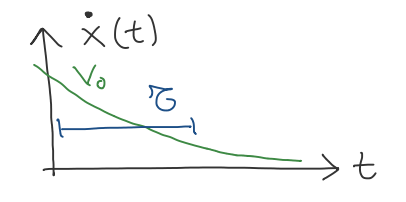
\includegraphics[width=\textwidth]{images/proiettile-gel-balitstico-2.png}
        \caption*{Soluzione completa gel}
    \end{subfigure}
\end{figure}

\subsection{Data la legge oraria, trovare la forza}
$r(t) = R, \Theta(t) = \Omega t$ \textbf{moto circolare uniforme}
$$\vec{r}(t) = r(t)\hat{r}\hspace{15pt}\hat{r} = \cos(\Theta(t))\hat{x} + \sin(\Theta(t))\hat{t}$$
$$\ddot{\vec{r}} (t) = [\ddot{r(t)} - r(t)\dot{\Theta}(t)^2]\hat{r} + [r(t)\ddot{\Theta}(t) + 2\dot{r}\dot{\Theta}(t)]\hat{\Theta}$$
Dalla legge oraria ho: $\dot{x}(t) = 0, \ddot{r}(t) = 0, \dot{\Theta} = \Omega, \ddot{\Theta}(t) = 0 \Rightarrow$ in questo caso $\ddot{\vec{r}}(t) = -R\Omega^2\hat{r}$.\\
La risultate $\vec{F}$ delle forze deve essere tale che $m\ddot{\vec{r}}(t) = \vec{F} \Rightarrow -mR\Omega^2\hat{r} = \vec{F} \Rightarrow \vec{F} = -mR\Omega\vec{r}$.\\
La forza è costante e sempre diretta verso lo stesso punto (\textbf{forza centrale} o  \textbf{forza centripeda}). Ottengo $\vec{F}$ solo per questa legge oraria.\\\\
Integrazione numeria delle equazioni del moto.

\subsection{Discretizzare la varibile temporale}
Calcolo al "primo ordine" ("metodo di eulero"), ci sono anche molti altri agloritmi come per esempio Runge-Kutta, la scelta
dipende dal problema.
$$t \to t_0, t_1, \dots, t_n \hspace{15pt} t_{i+1} - t_i = \Delta t \hspace{15pt}\vec{r}(t_i) = \vec{r}_i$$
$$\frac{d\vec{r}(t)}{dt}|_{t=t_i} \simeq \frac{\vec{r}_{i+1} - \vec{r}_i}{\Delta t} \hspace{20pt}\frac{d^2\vec{r}(t)}{dt}|_{t = t_i} \simeq \frac{\frac{\vec{r}_{i+1} - \vec{r}_i}{\delta t} - \frac{\vec{r}_i - \vec{r}_{i-1}}{\Delta t}}{\Delta t} = \frac{\vec{r}_{i+1} - 2 \vec{r}_i - \vec{r}_{i-1}}{\Delta t^2}$$
L'equazione di Newton diventa:
$$\vec{v}_i = \vec{v}_{i-1} + \Delta t \vec{F}_{i-1} / n \hspace{20pt}\vec{r}_i = \vec{r}_{i-1} + \Delta t \vec{v}_i$$
Servono 2 condizioni al bordo $\vec{F}_i$ può dipendere da $t_i, \vec{r}_i, \vec{v}_i$

\newpage
\section{Reazioni vincolari}
Estendiamo il modello del "punto materiale" all'interazione di corpi estesi in moto tralatorio
$\Delta \vec{r}_i = \Delta \vec{r}_2$ per ogni punto posso studiare una qualsiasi $\vec{r}(t)$
\begin{itemize}
    \item La \textbf{traslazione} può avvenire su una traiettoria curva, parleremo di \textbf{rotazione} più avanti.
    \item Consideriamo il \textbf{contatto} tra punti materiali, corpi estesi, superfici.
\end{itemize}
Le forze di contatto ("reazioni vincolari") non sempre hanno una espressione esplicita e vengono determinate imponendo dei vincoli alle 
equazioni del moto, ad esempio che un punto segua una data traiettora.
\begin{figure}[h!]
    \vspace{-10pt}
    \centering
    \begin{subfigure}[b]{0.25\textwidth}
        \centering
        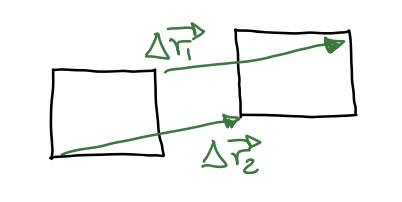
\includegraphics[width=\textwidth]{images/reazioni-vincolari-intro-1.png}
        \caption*{Traslazione punto materilae}
    \end{subfigure}
    \begin{subfigure}[b]{0.25\textwidth}
        \centering
        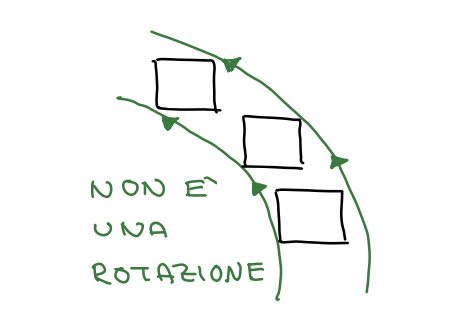
\includegraphics[width=\textwidth]{images/reazioni-vincolari-intro-2.png}
        \caption*{Rettilineo curvo}
    \end{subfigure}
    \begin{subfigure}[b]{0.4\textwidth}
        \centering
        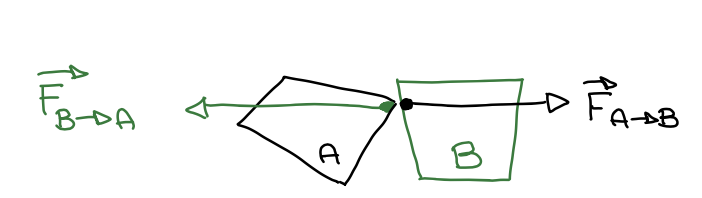
\includegraphics[width=\textwidth]{images/reazioni-vincolari-intro-3.png}
        \caption*{Contatto fra corpi}
    \end{subfigure}
\end{figure}
\begin{example} \label{es-rez-vin-1}
    $x(t) \equiv x_0$ 
\end{example}
\hspace{-15pt}La "terza legge di Newton" ("azione e reazione") stabilisce che $\vec{F}_{B\to A} = -\vec{G}_{A \to B}$
\begin{example} \label{es-rez-vin-2}
    Massa su una bilancia in presenza di forza peso.
    $$m\ddot{\vec{r}}(t) = -mg\hat{z} + \vec{F}$$
    In questo caso il \textbf{Vincolo} è: 
    $$\dot{\vec{r}}(t) = 0 \:\:\:\Rightarrow\:\:\: \vec{F} = +mg\hat{z}$$ 
    La bilancia misura $||-\vec{F}|| = mg$ (che noi chiamiamo comunemente peso).
\end{example}
\begin{example} \label{es-rez-vin-3}
    Massa su bilancia in ascesore accelerato.
    $$m\ddot{\vec{r}}(t) = -mg\hat{z} + \vec{F}$$
    Ciò che cambia ora è il suo \textbf{Vincolo} visto che si sta accelerando vesto l'alto: 
    $$\ddot{\vec{r}}(t) \equiv a \cdot \hat{z} \:\:\:\Rightarrow\:\:\: \vec{F}= m(a+g)\hat{z}$$
    La bilancia misura $||-\vec{F}|| = m(a+g)$.
    La bilancia allora misura una forza peso maggiore in un ascensore (stiamo usando l'equazione "al contrario").
\end{example}
\begin{note}
    Un punto materiale si "solleva", si "distacca" da una superfice quando la reazione vincolare va a zero.
\end{note}
\begin{figure}[h!]
    \vspace{-10pt}
    \centering
    \begin{subfigure}[b]{0.25\textwidth}
        \centering
        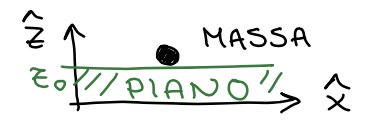
\includegraphics[width=\textwidth]{images/esempio-reazioni-vincolari-1.png}
        \caption*{Esempio \ref{es-rez-vin-1}}
    \end{subfigure}
    \begin{subfigure}[b]{0.25\textwidth}
        \centering
        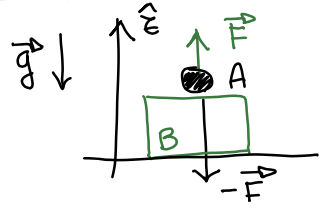
\includegraphics[width=\textwidth]{images/esempio-reazioni-vincolari-2.png}
        \caption*{Esempio \ref{es-rez-vin-2}}
    \end{subfigure}
    \begin{subfigure}[b]{0.2\textwidth}
        \centering
        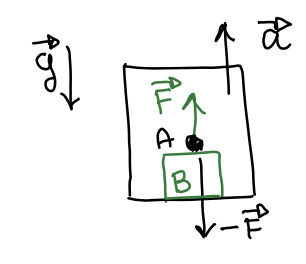
\includegraphics[width=\textwidth]{images/esempio-reazioni-vincolari-3.png}
        \caption*{Esempio \ref{es-rez-vin-3}}
    \end{subfigure}
\end{figure}
\hspace{-15pt}Scomponiamo la reazione vincolare nella direzione
\begin{itemize}
    \item ortogonale: "reazione normale" $\vec{N}$".
    \item parallelo: "forza di \textbf{attrito}" $\vec{F}_a$
\end{itemize}
\newpage
\begin{wrapfigure}[6]{r}{4cm}
    \centering
    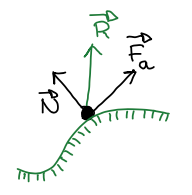
\includegraphics[width=2.7cm]{images/scomposizione-reazione-vincolare.png}
\end{wrapfigure}
ad una superficie. Con una superficie \textbf{liscia} abbiamo $\vec{F}_a = 0$, non c'è
movimento relativo al punto di contatto.
\textbf{Attrito statico}, $\vec{F}_a$ da determinare con vincoli. Condizione: $$||\vec{F}_a|| \leq \mu_s ||\vec{N}||$$
Differenza di velocità $\vec{v}$ al punto di contatto. \textbf{Attrito dinamico}:
$$\vec{F}_a = -\mu_a ||\vec{N}||\frac{\vec{v}}{||\vec{v}||}$$
$\mu_s, \mu_d$: coeff. di attrito, numeri primi.
$-\frac{\vec{v}}{||\vec{v}||}$ diretto in versione opposta alla velocità.

\begin{example}\label{es-rez-vin-4}
    Massa su un piano inclinato liscio e fisso.
    $$\hat{x}' = \cos\alpha \cdot \hat{x} - \sin\alpha \cdot \hat{z} \hspace{20pt}\hat{z}' = \sin\alpha \cdot \hat{x} + \cos\alpha \cdot \hat{z} \hspace{15pt} m\ddot{\vec{r}}(t) = -mg\hat{z} + \vec{N}$$
    \begin{itemize}
        \item Proietto lungo $\hat{z}'$: \hspace{15pt} $m\ddot{z}'(t) = -mg\cos\alpha + N$
        \item Proietto lungo $\hat{x}'$: \hspace{15pt} $m\ddot{x}'(t) = +mg\sin\alpha$.
    \end{itemize}
    Vincolo: $z'(t) = \cos t \hspace{10pt} \ddot{z}'(t) = 0\:\:\: \Rightarrow\:\:\: N = mg\cos\alpha \hspace{20pt} \ddot{x}'(t) = g \cdot \sin\alpha$\\
    Visto che $\sin\alpha < 1$ quindi l'accelerazione lungo il piano è $< g$.
\end{example}

\begin{example}\label{es-rez-vin-5}
    Massa ferma su piano inclinato scabro.
    $$m\ddot{z}'(t) = -mg\cos\alpha + N \hspace{20pt} m\ddot{x}'(t) = +mg\sin\alpha - F_{a}$$
    La scelta fra $-F_{a}$ o $+F_a$ è indifferente, l'unica cosa che cambia è nel risultato poi sarà diverso il segno di $F_a$, la coorenza da tenere è riguardante il disegno, se si disegna
    in una determinata direzione, si cerca di mettere il segno uguale.
    \begin{itemize}
        \item Vincolo: $z'(t) = \cos t \:\:\:\Rightarrow\:\:\: \ddot{z}'(t) = 0 \:\:\:\Rightarrow\:\:\: N = mg\cos\alpha$.
        \item Vincolo: $x'(t) = \cos t \:\:\:\Rightarrow\:\:\: \ddot{x}'(t) = 0 \:\:\:\Rightarrow\:\:\: F_a = mg\sin\alpha$
    \end{itemize}
    Qual'è il massimo valore di $\alpha$?
    $$||\vec{F}_a|| \leq \mu_s ||\vec{N}|| \:\:\:\Rightarrow\:\:\: mg\sin\alpha \leq \mu_s \cdot mg \cos\alpha \hspace{15pt} \tan\alpha \leq \mu_s \hspace{10pt} \alpha \leq \arctan\mu_s$$
\end{example}

\begin{example}\label{es-rez-vin-6}
    Massa scivola su piano inclinato scabro.
    $$m\ddot{z}'(t) = -mg\cos\alpha + N \hspace{20pt} m\ddot{x}'(t) = +mg\sin\alpha - F_{a}$$
    Vincolo: $z'(t) = \cos t \:\:\:\Rightarrow\:\:\: \ddot{z}'(t) = 0 \:\:\:\Rightarrow\:\:\: N = mg\cos\alpha$\\
    Forza di attrito dinamico: 
    $$F_a = \mu_{\alpha}N \:\:\:\Rightarrow\:\:\: m\ddot{x}'(t) = mg\sin\alpha - \mu_{\alpha} \cdot mg\cos\alpha \hspace{15pt} \ddot{x}'(t) = g(\sin g - \mu_{\alpha} \cdot \cos \alpha)$$
    Accelerazione costante, minore che senza attrito.
\end{example}

\begin{figure}[h!]
    \vspace{-10pt}
    \centering
    \begin{subfigure}[b]{0.25\textwidth}
        \centering
        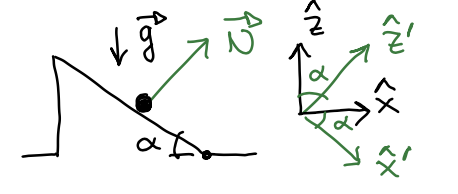
\includegraphics[width=\textwidth]{images/esempio-reazioni-vincolari-4.png}
        \caption*{Esempio \ref{es-rez-vin-4}}
    \end{subfigure}
    \hspace{20pt}
    \begin{subfigure}[b]{0.25\textwidth}
        \centering
        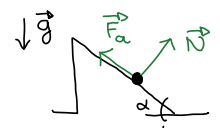
\includegraphics[width=\textwidth]{images/esempio-reazioni-vincolari-5.png}
        \caption*{Esempio \ref{es-rez-vin-5}}
    \end{subfigure}
    \hspace{20pt}
    \begin{subfigure}[b]{0.2\textwidth}
        \centering
        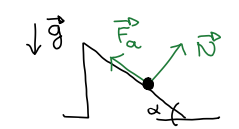
\includegraphics[width=\textwidth]{images/esempio-reazioni-vincolari-6.png}
        \caption*{Esempio \ref{es-rez-vin-6}}
    \end{subfigure}
\end{figure}